\chapter{实验设计}

\section{引言}
为验证我们的想法的可行性,需要进行实验或仿真。
进行实验关键是传感器的校准、实现夹爪的力控、相机的校准和识别算法的设计。
本章将介绍实验用到的设备和仪器,传感器的校准和力控的实现方法,
最后用仿真实验验证上文提出方案。

\section{实验装置}
该项目中用到的主要设备有单自由度高速夹爪一个,压力传感器一枚,
信号采集器一个,高速相机一台。实验装置如图 \ref{fig:4-1} 所示。

\begin{figure}[!ht]
  \centering
  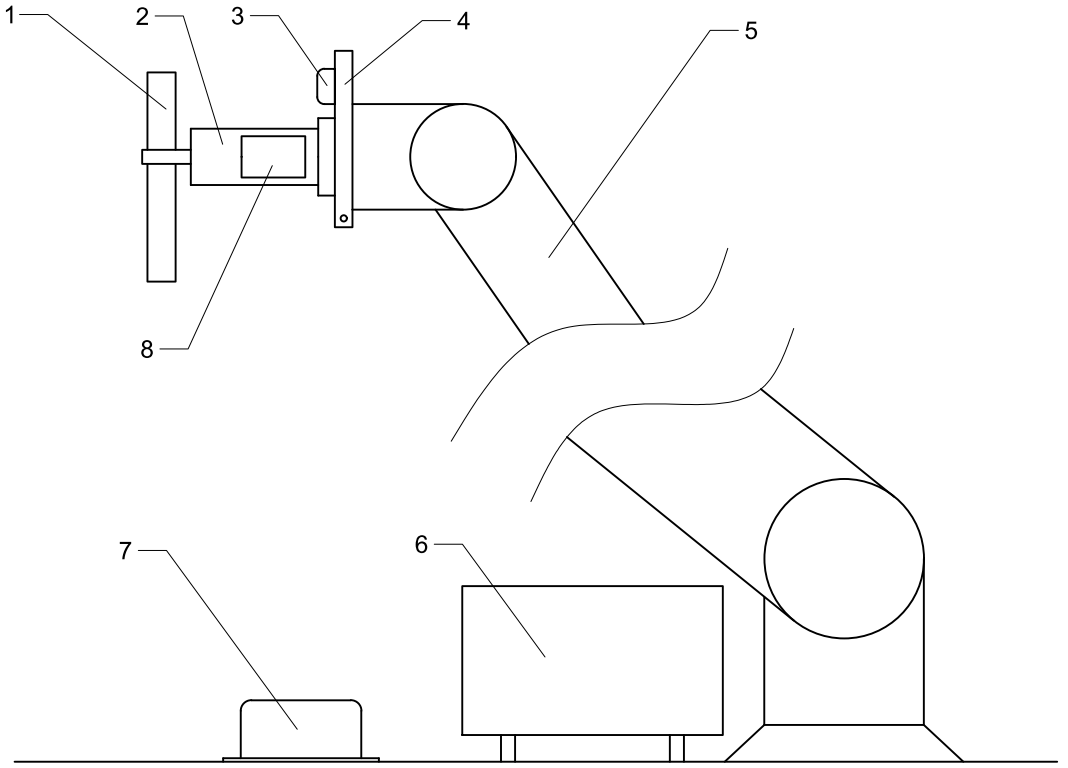
\includegraphics[scale=0.4]{chapter04/pic/4-1}
  \caption{实验装置简图}
  \label{fig:4-1}
  \vspace{-0.3cm}
\end{figure}

\vspace{-10pt}
\begin{center}
  \zihao{-5}
  1---被控物体; 2---高速夹爪; 3---Realsense相机; 4---相机支架; \\
  5---机械臂; 6---机械臂控制箱; 7---夹爪控制器; 8---数据采集卡;
\end{center}

图中相机固定在相机支架上,同高速夹爪一起固定在机械臂末端;
数据采集卡固定在夹爪上;薄膜式压力传感器贴在夹爪内侧,
通过设计的电路与数据采集卡连接。
按照各设备要求连接通信线路,夹爪连接控制器,
控制器和相机均通过 USB 线缆连接上位机;
机械臂用专用线缆连接控制箱,控制箱通过网线连接上位机。

\section{压力传感器的校准}
实验使用的压力传感器类型为:宇博智能 RFP601 型薄膜压力传感器,量程为500g,
是一款压阻式单点压力传感器, 响应时间为微秒级。
图 \ref{fig:4-2} 所示是传感器的电阻—压力曲线图。
实验使用的信号采集器为恒凯 USB 数据采集卡,
提供 12 位 AD采集通道支持 0~3.3V 模拟输入,最高采样频率可达 100Ksps.

\begin{figure}[!ht]
  \centering
  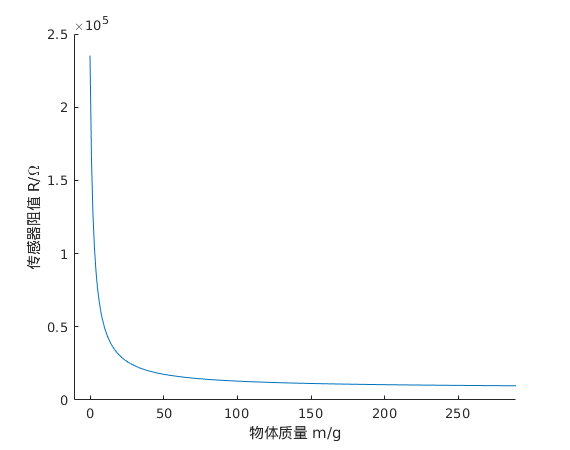
\includegraphics[scale=0.7]{chapter04/pic/4-2}
  \caption{压力传感器质量---电阻曲线}
  \label{fig:4-2}
  \vspace{-0.3cm}
\end{figure}

该传感器的电阻和压力曲线可近似用反比例函数表示。即式(\ref{equ:4-1})。
设计如图\ref{fig:4-3}所示电路图,图中电源电压为 3.3V, $R_0$ 为固定电阻,
压敏电阻 $R$ 为传感器。通过 A 点电压值可以计算传感器的阻值,即式(\ref{equ:4-2})。
代入式(\ref{equ:4-1})即可得到压力与 A 点电压的关系式(\ref{equ:4-3})。

\vspace{-10pt}
\begin{equation}
  \label{equ:4-1}
  R = \frac{{k'}}{{m + c'}} + a'
\end{equation}
\vspace{-30pt}

\begin{equation}
  \label{equ:4-2}
  R = (\frac{V}{u} - 1) \cdot {R_0}
\end{equation}
\vspace{-30pt}

\begin{equation}
  \label{equ:4-3}
  m = \frac{{c - ku}}{{au - 1}}
\end{equation}

式中 $R_0$ 为固定电阻阻值 $(\Omega )$ , R 为压敏电阻阻值 $(\Omega )$ ,
$m$ 为传感器受到的力 $(g)$ , $V$为电源电压, $u$ 为 $A$ 点电压值,
$a'$, $c'$, $k'$, $a$, $c$ , $k$ 均为与电阻 $R$ 有关的常数。

\begin{figure}[!ht]
  \centering
  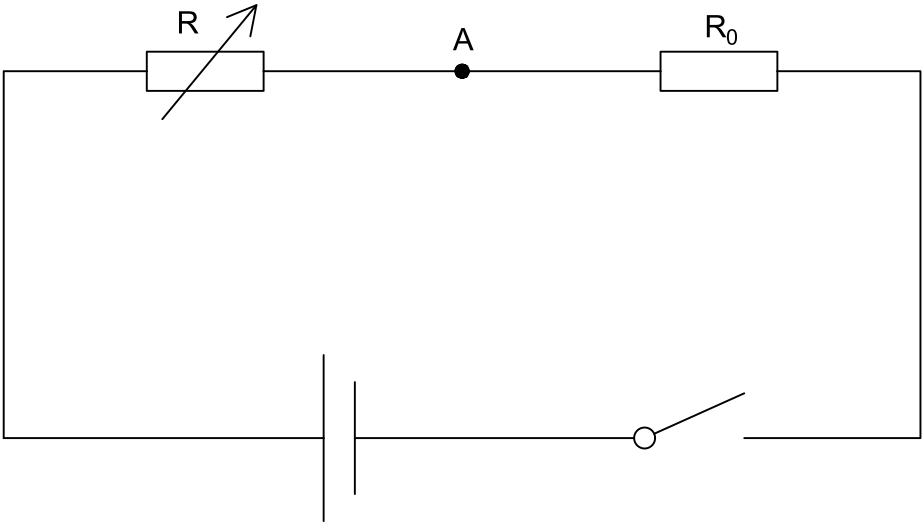
\includegraphics[scale=0.3]{chapter04/pic/4-3}
  \caption{数据采集电路图}
  \label{fig:4-3}
  \vspace{-0.3cm}
\end{figure}

由式(\ref{equ:4-3})可知, $u$ 趋近于 0 时传感器精度过低,对受力响应过大;
$u$ 趋近于 $cV$ 时传感器灵敏度过低。适当调整固定电阻的阻值可以改善传感器效果,
经实验确定该项目拟用阻值为 $R=10k\Omega$ 的固定电阻。

多次测量不同压力下 A 点的电压值,绘制散点图如图(\ref{fig:4-4})所示,利用 Matlab 进行
拟合,拟合结果确定式(\ref{equ:4-3})中的参数为
$c = − 6.431$ , $ k = 10.72 $ , $a = 0.4967$ ,置信概率为 $95\%$ 。

\begin{figure}[!ht]
  \centering
  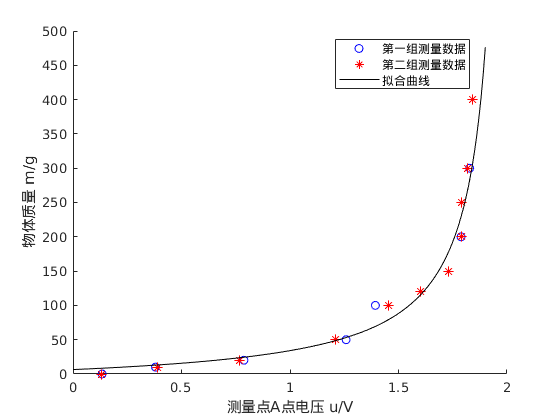
\includegraphics[scale=0.63]{chapter04/pic/4-4}
  \caption{采集数据散点图与拟合图}
  \label{fig:4-4}
  \vspace{-0.3cm}
\end{figure}

\section{高速夹爪的伺服控制与力控}
实验中使用的夹爪为增广智能科技 RM-MGBD--11-14-L 微型伺服夹爪.
控制器与夹爪通信时间约为 5ms, 即发送运动信息和读取夹爪位置需要 5ms 的时间,
由于力控不需要夹爪位置反馈, 故伺服周期应大于 5ms,
考虑到读取传感器数据和程序运行等需要一定的时间, 我们将伺服周期设为 8ms.

在力控实验中经过多次参数调整后,我们最终采用的 PD 控制器参数为
$k_p = 0.0008$ , $k_i = 0.0004$, $k_d = 0.0008$ 。
图 \ref{fig:4-5} 和图 \ref{fig:4-6} 分别展示了使用改良PD控制算法后系统的输出信号
相对恒定输入信号和正弦输入信号的跟踪效果。


\begin{figure}[!h]
  \centering
    \subfloat[压力变化曲线]{
      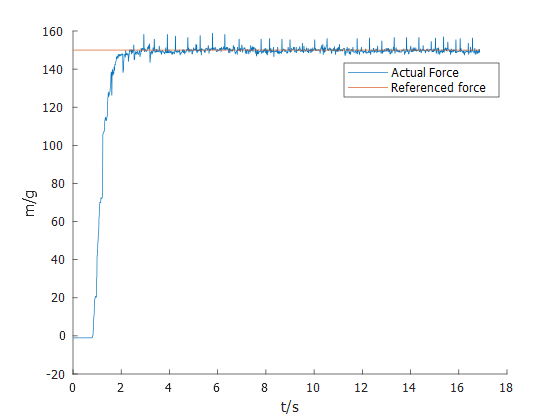
\includegraphics[width=7.2cm]{chapter04/pic/150}
    }
    \hspace{0pt}
    \subfloat[夹爪位置信号]{
      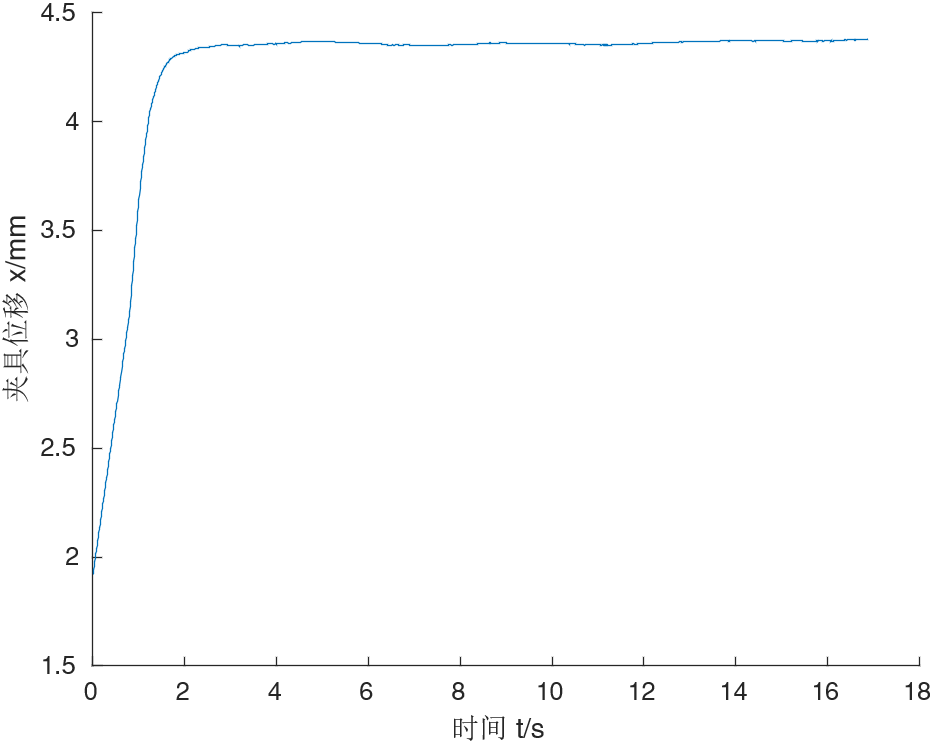
\includegraphics[width=7.2cm]{chapter04/pic/150_x}
    }
  \caption{\label{fig:4-5}阶跃信号下的压力和夹爪位置信号曲线}
  \vspace{-0.3cm}
\end{figure}

% \begin{figure}[!ht]
%   \centering
%   \includegraphics[scale=0.70]{chapter04/pic/4-5}
%   \caption{PID控制下系统阶跃响应}
%   \label{fig:4-5}
%   \vspace{-0.3cm}
% \end{figure}

图\ref{fig:4-5}a)可以展示了 改进后的控制器在阶跃输入信号下的控制效果。
最终压力均值保持在期望值 150 g左右,输出信号的波动主要原因是传感器误差,
波动范围在可接受范围内。
调节时间约为 2s ,这并不影响我们的实验的控制效果,因为实际实验中,
初始状态下夹爪是抓紧工具的,而在运动过程中压力变化虽然很频繁但是增量不大,
所以实验过程中压力信号的改变幅度不会过大,压力信号与实际压力值相差也较小,
因此图示的调节时间是可以接受的。
图\ref{fig:4-5}b)展示了在这一过程中控制器对夹爪发送的位置命令,
可以看到位置信号和压力信号的变化趋势趋于一致,
而且在压力值到达150g附近时位置命令保持稳定,只有轻微的振动,
这也说明了压力的波动是由于传感器造成的。



\begin{figure}[!h]
  \centering
    \subfloat[压力变化曲线]{
      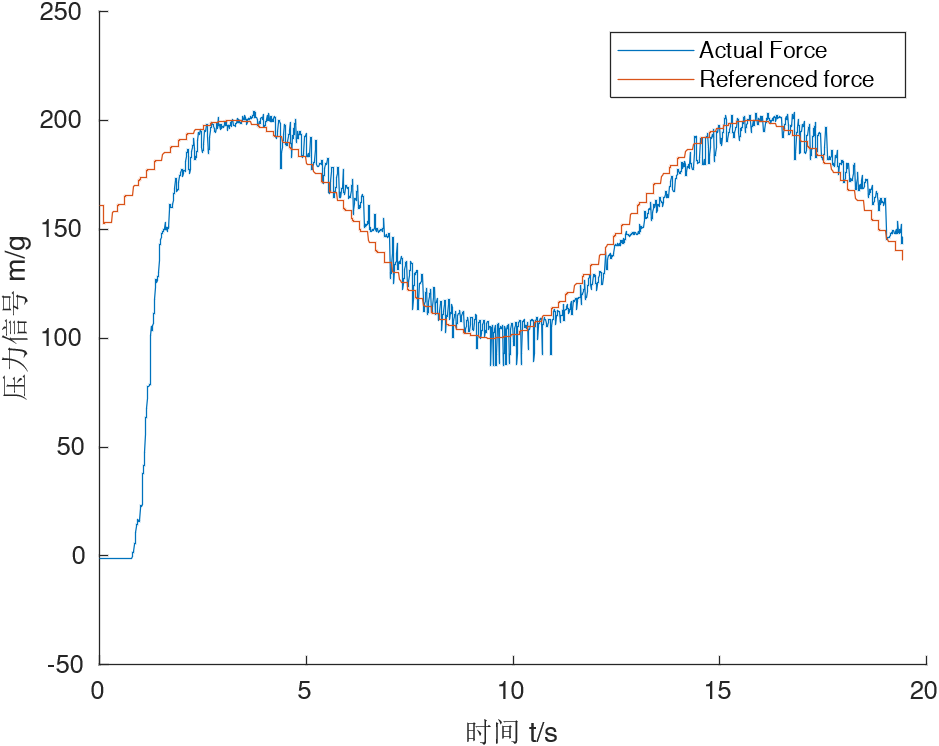
\includegraphics[width=7.2cm]{chapter04/pic/sin}
    }
    \hspace{0pt}
    \subfloat[夹爪位置信号]{
      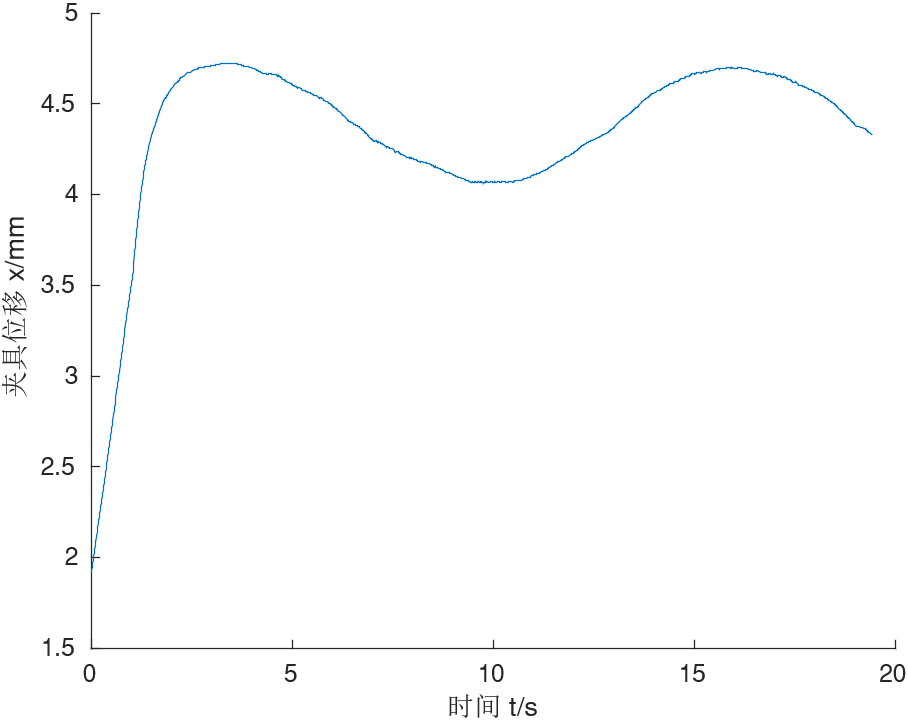
\includegraphics[width=7.2cm]{chapter04/pic/sin_x}
    }
  \caption{\label{fig:4-6}正弦信号下的压力和夹爪位置信号曲线}
  \vspace{-0.3cm}
\end{figure}

% \begin{figure}[!ht]
%   \centering
%   \includegraphics[scale=0.70]{chapter04/pic/4-6}
%   \caption{PID控制下输出量对正弦信号的跟踪性能}
%   \label{fig:4-6}
%   \vspace{-0.3cm}
% \end{figure}

从图\ref{fig:4-6}a)可以看出在信号持续变化的情况下 PD 控制器的控制效果也符合预期。
长时间的控制下,虽然传感器误差会有一定的波动,但是系统保持稳定,
实际压力均值持续跟随正弦输入信号,没有明显的误差,输出信号的波动范围在可接受范围内。
同理调节时间并不影响我们的实验的控制效果。
结合这两个实验可以说明 PD控制是可以满足我们的控制需求的。
图\ref{fig:4-6}b)展示了在该过程中控制器的位置指令,
可以看到位置信号和压力信号的变化趋势趋于一致。
位置信号不是严格的正弦信号, 这是因为传感器采集的电压信号转化为压力信号不是线性的。
所以在不同压力大小下产生同样压力差所需的位移大小不同,
在位置信号图上,压力在极大值和极小值附近的变化幅度有差异。


\section{仿真实验}
为验证上文提出的想法的可行性,我们设计了仿真实验。
采用表 4-1 所示的物理参数带入 Simulink 模型进行仿真实验,
观察实验现象并分析仿真结果。虽然仿真实验中数据可能会过于理想,
但是这在某种程度上也能佐证方案的合理性。
在这次仿真试验中,我们通过直接给夹爪运动副施加控制力,即力控是理想的。
这样可以证明我们推导的动力学模型和控制模型理论上是正确的。

\begin{table}[!h]
\centering
\caption{仿真实验参数取值表\label{tab:4-1}}
\begin{tabular}{@{}ccccccccc@{}}
\toprule[1pt]
 \makebox[3.5em][c]{$h_d/mm$}   & \makebox[2.5em][c]{$m/g$}  &
 \makebox[2.5em][c]{$\mu$}      & \makebox[2.5em][c]{$\sigma$}  &
 \makebox[2.5em][c]{$k$}        & \makebox[2.5em][c]{$\lambda$}  &
 \makebox[2.5em][c]{$\alpha_a$} & \makebox[2.5em][c]{$\alpha_c$}  &
 \makebox[2.5em][c]{$\alpha_c$} \\ \midrule

20       &  12       &  0.5     &  0.3    &2        &  6        &
20      &  20     &  20    \\
\bottomrule[1pt]
\end{tabular}
\end{table}


工具下落过程中的位置变化曲线如图 \ref{fig:4-7} 所示。从图中可以看出,工具的位移
曲线很好地跟随了参考模型信号,并且最终停在了目标位置 $h = 20 mm$ 处。由此可
知,模型参考自适应控制系统能够达到理想的控制效果,本次实验中在并未给出具
体的摩擦参数以及物体质量的情况下,平行指夹具仍然成功地控制工具运动到了目
标位置。


\begin{figure}[!ht]
  \centering
  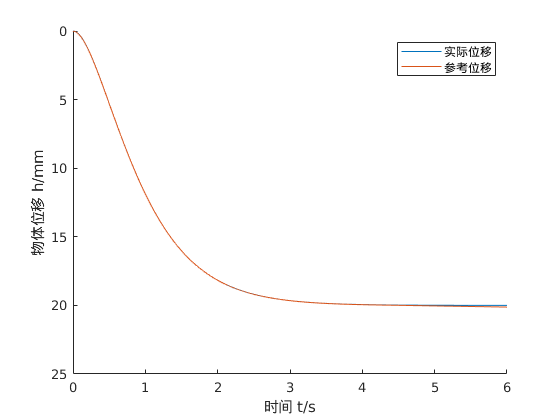
\includegraphics[width=12cm]{chapter04/pic/h_f}
  \caption{工具位移曲线}
  \label{fig:4-7}
  \vspace{-0.3cm}
\end{figure}


夹具位置信号的变化曲线如图 \ref{fig:4-8}a) 所示。图中 t = 0 s 附近,
即仿真刚开始时的一小段突变是由于初始状态下夹具与工具之间并未紧密接触,
工具的快速下落与参考模型中的输出信号的广义偏差很大,所以夹具位移突变很大。
时间在0s 到 2s左右夹具位置几乎无变化, 这是因为在这段时间内夹具的运动可近似为匀速运动,
而在0s左右时,控制器已经通过实时的广义误差估计出了摩擦系数,
所以这段时间内夹具只需要保持在固定位置即可实现工具的匀速运动。
时间在 2s 到 2.5s 附近夹具位置变化频繁,
这是因为工具速度发生变化,运动过程中需要保持工具运动曲线跟踪参考曲线,所以夹具运动频繁。
另一方面,由于该仿真模型中夹具和工具都接近刚体,导致两模型的碰撞效果明显。
在 3s 之后,夹具位置变化趋于稳定,说明工具运动减慢,并逐渐停止。
由于存在少许的超调量,广义误差 s 一直小于零,所以压力应该持续增大,导致夹具位移持续增大。

% \begin{figure}[!ht]
%   \centering
%   \includegraphics[scale=0.6]{chapter04/pic/4-8}
%   \caption{夹具位移曲线}
%   \label{fig:4-8}
%   \vspace{-0.3cm}
% \end{figure}

压力传感器记录的数据如图 \ref{fig:4-8}b) 所示。压力的变化趋势与夹具位移一致,
这是因为接触模型中形变量与弹性力成正比。
为了更好的仿真效果,需要修正夹具模型,将其修改为刚度系数较小的弹性体。

% \begin{figure}[!ht]
%   \centering
%   \includegraphics[scale=0.6]{chapter04/pic/4-9}
%   \caption{工具单侧所受正压力变化曲线}
%   \label{fig:4-9}
%   \vspace{-0.3cm}
% \end{figure}

\begin{figure}[!h]
  \centering
    \subfloat[夹具位移曲线]{
      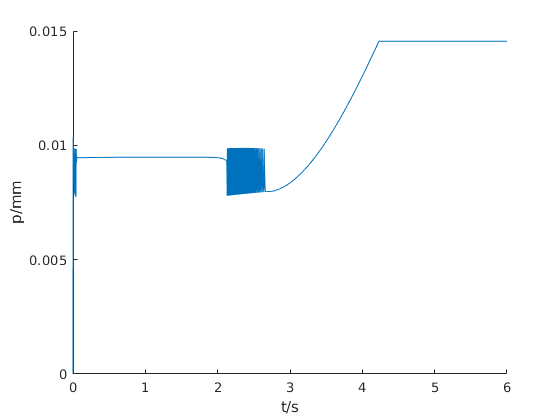
\includegraphics[width=7.2cm]{chapter04/pic/p_f}
    }
    \hspace{0pt}
    \subfloat[压力变化曲线]{
      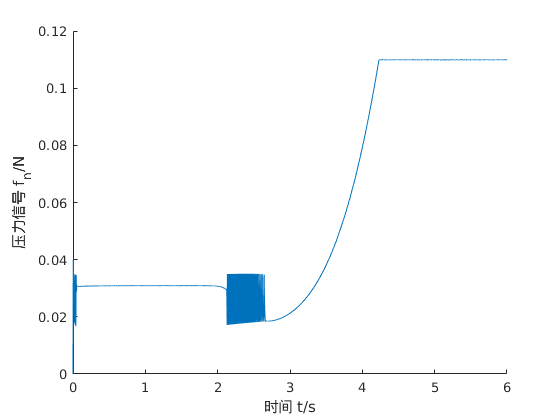
\includegraphics[width=7.2cm]{chapter04/pic/fn_f}
    }
  \caption{夹具位移及受力曲线图}
  \label{fig:4-8}
  \vspace{-0.3cm}
\end{figure}

通过这一仿真实验,我们可以确保上文推导的工具动力学方程(式 \ref{equ:2-3})的正确性,
以及适应性控制方程(\ref{equ:2-7})和调参规律(\ref{equ:2-8})可以保证跟踪误差的收敛,
可以精准控制物体下落的轨迹。


\section{添加力控的仿真实验}
在实际实验过程中,理想的力控是难以实现的。
为了更好的仿真效果, 我们需要修改仿真模型,
我们在图 \ref{fig:3-5} 的基础上为夹爪添加了一个弹簧模型, 以模拟实际场景中的缓冲垫片。
并且直接对运动副施加控制力的方案被修改为对运动副施加位移控制,
以模拟控制器对夹爪发送的控制指令。
然后添加PD控制子模块, 并调整合适的参数,以模拟真实场景中的力控效果。
最终机械系统子模块的仿真模型图如下图 \ref{fig:mech_x} 所示。

\begin{figure}[!ht]
  \centering
  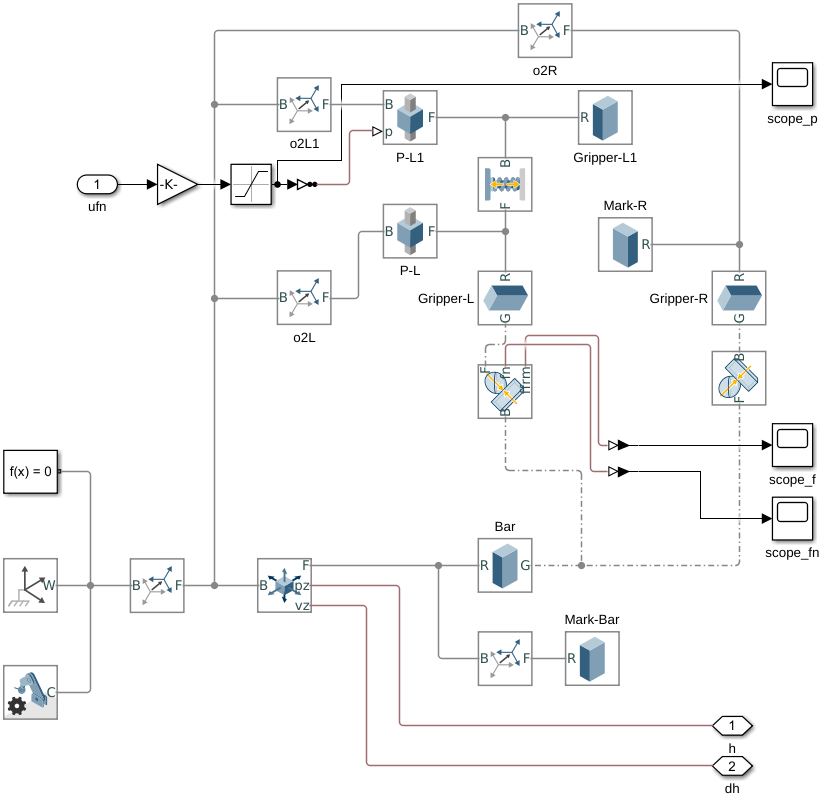
\includegraphics[width=13cm]{chapter04/pic/mech_x}
  \caption{\label{fig:mech_x}
    添加力控的机械系统模块}
  \vspace{-0.3cm}
\end{figure}

再次重复上述实验, 工具的位移曲线如 \ref{fig:h_x} 所示。
从图中可以看出,工具的位移曲线依旧能跟随了参考模型信号,
虽然会出现频繁停止和突然运动的现象,但是工具最终依然停在了目标位置 $h = 20 mm$ 处。
由此可知, 我们使用的控制方案能够达到理想的控制效果。
但是这次实验中也暴露出一些问题, 比如在快达到目标位置但还未达到时,
控制器会累计误差, 直到误差足够大时, 夹爪会张开让工具开始运动,
如果夹爪速度不够快或者控制器响应速度不够高, 那么工具有可能会超过期望位置后才被停止。
这一问题显然可以通过加快系统响应速度来解决, 另一方面, 也可以通过添加一容差区间来解决。
比如让控制器检测到广义误差小到可接受范围内时, 即认为工具已经达到目标位置, 操作结束。
图中工具运动会突然停止再突然运动,这是因为软指接触中,手指上的垫片过软。
由于缓冲效果明显,压力传感器检测到的力变化幅度较小,手指慢慢张开后工具开始下落;
而检测到广义误差过大后,控制器发送指令让手指闭合,手指闭合过程对工具的力被缓和,
工具在手指闭合到既定位置时还能下落一定距离。
这将使得自适应控制器错误的将摩擦系数估计得过小。
因此在下次张开手指时,控制器计算的夹具位移应该比理论值更小, 也使得工具停止时间增长。
另一方面,这也导致了夹具位置变化频繁,
以此保证工具连续运动过程中工具运动曲线能更好的跟踪参考曲线。

\begin{figure}[!ht]
  \centering
  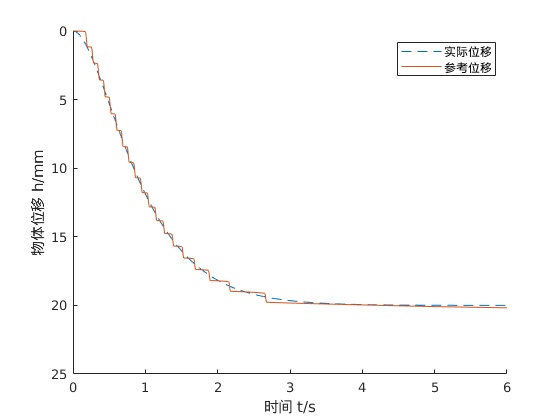
\includegraphics[width=12cm]{chapter04/pic/h_x}
  \caption{\label{fig:h_x}
    工具位移曲线}
  \vspace{-0.3cm}
\end{figure}


夹具位置信号的变化曲线如图 \ref{fig:4-11}a) 所示。
图中夹具位置变化频繁,这是由于工具不连续的运动状态导致的,
运动过程中需要保持工具运动曲线跟踪参考曲线,所以夹具运动频繁。
在我们的实验中,我们发现了夹爪手指垫片的刚度系数和工具运动连续程度的定性关系。
当垫片或胶皮过软,即刚度系数过小时,工具每次停止的时间越长,每段下落距离越长,
在工具位移曲线图上表现为阶梯状越明显。
反之运动越连续, 运动曲线对参考曲线的跟踪性能越好。
这并不难理解, 刚度越低时夹具要使工具开始运动或停止运动需要产生的位移越大,
在其他条件如夹具运动速度,PD控制系数等参数相同的情况下, 工具对夹具位移的响应越慢,
因此运动会断断续续, 而且每段运动过程中下落和停止的时间均会增长。
但是, 刚度也不能过高, 因为这需要系统具有更快的响应速度和更精准的力控。
否则可能造成系统震荡, 或夹爪由于受力过大而保护性停止。

\begin{figure}[!h]
  \centering
    \subfloat[夹具位移曲线]{
      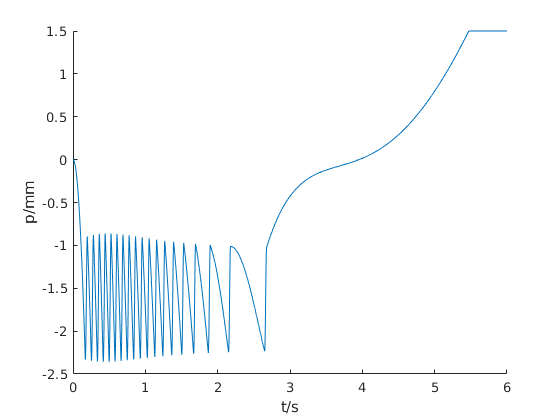
\includegraphics[width=7.2cm]{chapter04/pic/p_x}
    }
    \hspace{0pt}
    \subfloat[压力变化曲线]{
      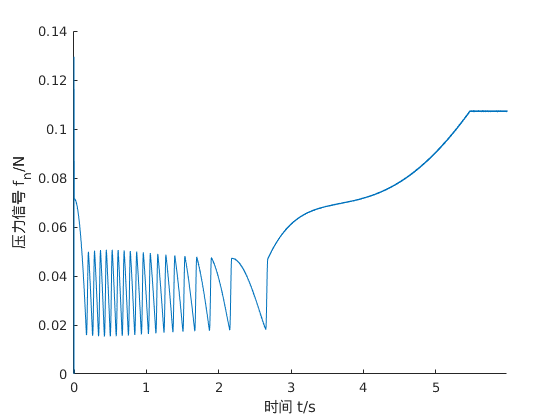
\includegraphics[width=7.2cm]{chapter04/pic/fn_x}
    }
  \caption{夹具位移及受力曲线图}
  \label{fig:4-11}
  \vspace{-0.3cm}
\end{figure}

同样,在这次实验中夹具位移也会在物体停止后持续增大。
这也由于超调量使得广义误差大于零且一直累加导致的。
为了防止位移信号持续增大而使得信号超过阈值造成机器停止等问题,
我们人为添加了饱和模块,以限制输出的位置指令。


\section{本章小结}
为验证单自由度机器人手进行被动在手操作的实现方法设计了一套实验方案。
分析了压力传感器输出特性,设计测量电路,校准了传感器。
完成了高速夹爪的伺服控制和力控实验。
最后使用 Matlab/Simulink 中的多体动力学模块进行仿真,
分析了仿真结果,论证了使用模型参考自适应控制算法实现物体在手操作的合理性。

